\documentclass[fleqn,10pt]{wlscirep}
\usepackage[utf8]{inputenc}
\usepackage[T1]{fontenc}
\usepackage{type1cm}% CM-Fonts including math fonts in all sizes. Repairs 'Font shape OML/cmm/m/it in size <...> not available'.
\usepackage{ae,aecompl}% Repairs 'Font shape T1/cmr/m/n in size <...> not available'.
\usepackage{microtype}
\usepackage{hyperref}
\usepackage{tikz}
\usetikzlibrary{shapes,arrows}
\hypersetup{colorlinks,allcolors=black}


% Manuscript draft.
%\usepackage{lineno}
%\linenumbers

% Figures and tables.
\usepackage{booktabs}
\usepackage{tabularx}
\usepackage{multirow}
\usepackage{multicol}

\usepackage{graphicx}
\DeclareGraphicsRule{.ai}{pdf}{*}{}% Handle .ai files as .pdf files.
\DeclareGraphicsExtensions{.pdf,.ai,.jpg,.png}
\setkeys{Gin}{pagebox=artbox}% Use artbox instead of mediabox default. Options: mediabox, cropbox, bleedbox, trimbox, artBox. (shell: pdfinfo -box <pdf-file>)
\graphicspath{{../sdata22-scientific-text-reuse-corpus-figures/}}

\newcommand{\bsfigure}[3][1.0]{%
  % # scale
  % #2 file name
  % #3 caption
  \begin{figure}[tb]
    \centerline{\includegraphics[scale=#1]{#2}}
    \vspace{-1ex}\caption{\small#3.}\label{#2}
    % Alternative.
    % \ifx#3\empty\else\vspace{-1ex}\caption{\small#3.}\label{#2}\fi
    \vspace{0.5ex}\vglue 0ex plus 0.5ex minus 1ex
  \end{figure}}



% Itemization.
\newcommand{\Ni}{(1)~}
\newcommand{\Nii}{(2)~}
\newcommand{\Niii}{(3)~}
\newcommand{\Niv}{(4)~}
\newcommand{\Nv}{(5)~}


% Commenting.
\newcommand{\todo}[1]{{\color{blue}#1}}

\newif\ifbscomment
\bscommentfalse
\bscommenttrue% Show comments.

\RequirePackage{xcolor}
\RequirePackage{soul}
\setstcolor{blue}

\newsavebox\bscombox
\newcommand{\bscom}[3][]{%
    % #1 Optional comment.
    % #2 Original text.
    % #3 Replacement text.
    \sbox{\bscombox}{\fontsize{8}{9}\selectfont#1#2#3}
    \noindent
    \st{#2}{\selectfont
        \color{blue}#3\ifx\\#1\\\else{\color{violet}[#1]}\fi
    }
}


% Paper commands.
\usepackage{xspace}
\newcommand{\webisReuseCorpus}{\texttt{Webis-STEREO-21}\xspace}


% Global settings.
\raggedbottom % \flushbottom


%%%%%%%%%%%%%%%%%%%%%%%%%%%%%%%%%%%%%%%%%%%%%%%%%%%%%%%%%%%%%%%%%%%%%%%%
\begin{document}


%\title{A Dataset on Scientific Text Reuse in Open Access Publications}
%\title{Scientific Text Reuse in Open Access Publications}
\title{STEREO: Scientific Text Reuse in Open Access Publications}

\author[1,*]{Lukas Gienapp}
\author[1]{Wolfgang Kircheis}
\author[1]{Bjarne Sievers}
\author[2]{Benno Stein}
\author[1,*]{Martin~Potthast}
\affil[1]{Leipzig University, Text Mining and Retrieval Group, Leipzig, DE-04109, Germany}
\affil[2]{Bauhaus-Universität Weimar, Web Technology and Information Systems Group, Weimar, DE-99423, Germany}
\affil[*]{corresponding authors: Lukas Gienapp, Martin~Potthast~(\textless first\textgreater.\textless last\textgreater@uni-leipzig.de)}


\begin{abstract}
We present the \webisReuseCorpus dataset, a massive collection of \textbf{S}cientific \textbf{Te}xt \textbf{Re}use in \textbf{O}pen-access publications. It contains more than 91~million cases of reused text passages found in 4.2~million unique open-access publications. Featuring a high coverage of scientific disciplines and varieties of reuse, as well as comprehensive metadata to contextualize each case, our dataset addresses the most salient shortcomings of previous ones on scientific writing. \webisReuseCorpus allows for tackling a wide range of research questions from different scientific backgrounds, facilitating both qualitative and quantitative analysis of the phenomenon as well as a first-time grounding on the base rate of text reuse in scientific publications.
\end{abstract}

% keywords can be removed
%\keywords{First keyword \and Second keyword \and More}

\maketitle

\input{sdata22-scientific-text-reuse-corpus-part1}
\section*{Methods}
\label{sec:method}

%%% NOTES. (journal instructions)
%%%
%%% The Methods should include detailed text describing any steps or procedures used in producing the data, including full descriptions of the experimental design, data acquisition assays, and any computational processing (e.g. normalization, image feature extraction). See the detailed section in our submission guidelines for advice on writing a transparent and reproducible methods section. Related methods should be grouped under corresponding subheadings where possible, and methods should be described in enough detail to allow other researchers to interpret and repeat, if required, the full study. Specific data outputs should be explicitly referenced via data citation (see Data Records and Citing Data, below). Authors should cite previous descriptions of the methods under use, but ideally the method descriptions should be complete enough for others to understand and reproduce the methods and processing steps without referring to associated publications. There is no limit to the length of the Methods section. Subheadings should not be numbered.


To compile a dataset on text reuse in scientific writing, three things are required: a large collection of scientific publications; detailed metadata for each of these publications; and a scalable, yet accurate method for detecting reuse between the compiled texts. This section formally introduces all three of these components. Our pipeline and its individual steps are depicted in Figure~\ref{fig:pipeline} for reference. Note that text reuse detection is typically implemented as a bipartite process of source retrieval to identify candidate pairs of documents, followed by text alignment to identify reused portions of text between both candidate documents \cite{stein:2007d}.


\subsection*{Publication Acquisition, Preprocessing and Metadata}\label{sub:data}

Before the detection of scientific text reuse at scale can commence, a large amount of scientific publications and detailed metadata has to be collected. We assemble such data in the five steps document selection, plain text extraction, text preprocessing, meta data acquisition, and meta data standardization.

For raw document selection, we make use of the CORE dataset \cite{knoth:2012}, one of the largest collections of open access academic publications, obtained from more than 12,000 data providers. First, we identify the 6,015,512 unique open-access DOIs in the CORE dataset dump from March~1st,~2018. Since the plain texts extracted from the publications' PDF files as supplied by the CORE data are of highly varying quality, and since no structural annotations (such as markup for citations, in-text references, section annotations) are available, we opted to obtain the original PDF files of the identified open access DOIs from various openly accessible repositories.

Plain text extraction was then repeated on the acquired PDF files using the standardized state-of-the-art toolchain GROBID \cite{lopez:2015}. The extracted texts are preprocessed as follows: For each document, abstract and main text paragraphs are extracted as indicated by the content tags provided by GROBID; in-text references, tables, and figures are omitted. We choose to further drop the bibliographical data, special characters, and numerical characters to reduce the amount of false positives for the subsequent text alignment step. Since the retrieval models underlying the text alignment detection compute the word overlap between document passages, standardized or meta text fragments such as citations, numbers, author names, affiliations, and references exponentially increase the set of passages matched between documents that otherwise may not share text. A minimum of 1,000 and a maximum of 60,000 whitespace-separated words is imposed as an effective heuristic to filter common plain text extraction errors. Overall, we obtained and extracted clean plain text for 4,267,166 documents~(70\% of the original CORE dataset).

Given this set, we cross-check and supplement the metadata provided by CORE with additional data from the Microsoft Open Academic Graph \cite{tang:2008,sinha:2015}, which features fields-of-study annotations for a wide set of publications. Since the annotated disciplines do not follow a hierarchical scheme, and since they are of differing granularity per publication (e.g., ``humanities'' as a whole vs.\ ``chemical solid-state research'' as a subfield of chemistry), we manually map the classification found in the Microsoft Open Academic Graph to the standardized, hierarchical \textit{DFG Classification of Scientific Disciplines, Research Areas, Review Boards and Subject Areas} \cite{dfg:2016}.\footnote{We opt to replace the term \textit{review board} as used in the DFG classification with the more conventional denomination \textit{field of study}.}



\subsection*{Text Reuse Detection in Large Document Collections}

Given the large collection of plain texts, a text reuse detection approach is applied  to identify reused passages between pairs of texts. At heart, the detection of text reuse boils down to the task of {\em text alignment} \cite{potthast:2013e}: Given two documents~$d$ and~$d'$, determine the set $R_{d,d'}$ of all pairs of reused text passages $(t, t')$, where $t\subseteq d$ and $t' \subseteq d'$. 

When given a set of documents~$D$, the computational complexity of detecting the set $R_D$ of all pairs of reused text passages among all pairs of documents, $\{(d, d')\mid d, d'\in D\}$, grows quadratically with the document count, {$|D|$}. If an exhaustive comparison exceeds the available computing capacity, a source retrieval step has to be carried out first \cite{hagen:2015e,hagen:2017e}: Given a document~$d$ and a document collection~$D$, a subset $D_d\subseteq D$ of candidate documents is retrieved containing those documents $d'\in D_d$ whose likelihood of sharing a reused text passage with~$d$ is sufficiently high. The size $|D_d|$ for a given document~$d$ varies dependent on how many documents in~$D$ have a sufficiently high reuse likelihood, but is expected to be $|D_d| \ll |D|$. Note that the estimation of a reuse likelihood for all pairs $\{(d, d')\mid d, d'\in D\}$ can be operationalized with linear time complexity in~$|D|$, e.g., by using locality-sensitive hashing \cite{stein:2019c}.

Source retrieval introduces an error in terms of lower recall, i.e., missed pairs of reused passages that would have been detected by an exhaustive text alignment of every document pair. The goal of source retrieval therefore is to closely approximate the recall of an exhaustive comparison while minimizing the sum of the sizes of retrieved candidate documents $\sum_{d\in D} |D_d|$, i.e., the computing capacity actually expended. Altogether, to detect reused text passages in~$D$, we retrieve for each $d \in D$ the set $D_d$ of candidate documents and compute for each $d'\in D_d$ the set of reused text passages $R_{d,d'}$. The union of all detected passages is used as an approximation of~$R_D$.



\subsection*{Source Retrieval}

The source retrieval component of our pipeline, i.e., the computation of $D_d$ for a given $d$, is operationalized by treating text reuse as a locally bounded phenomenon. Candidate pairs are presumed to be identifiable by comparing text passages between two documents. If the similarity is sufficiently high for at least one combination of passages between two documents $d, d'$, then $d'$ is considered a candidate for $d$. To achieve high scalability, we apply a locality-sensitive hash function~$h$ to each passage~$t$ in a document~$d$, thus representing each document as a set of hash values~$h(t)$. The similarity between two passages $t,t'$ is then approximated by the extent of overlap between their hash sets, $|h(t)\cap h(t')|$. Thus, a document $d'$ is considered a candidate source of text reuse for a document $d$, if at least one of their passage-level hash sets intersects \cite{stein:2019c}: $\exists t \subseteq d \ \exists t' \subseteq d' : h(t) \cap h(t')\neq\emptyset$. 

In our pipeline, the documents are first divided into consecutive passages of $n$~terms, which in turn are each embedded using a bag-of-words representation, i.e., as their term occurrence vector. To find matching passages between two documents, MinHash \cite{broder:97} is chosen as hashing scheme for~$h$. For each passage vector, multiple individual hash functions are applied to each element, and the minimum hash value of each pass is saved, yielding the set minimum hashes for a passage. It can be shown that, for~$m$ individual hashes per passage, two texts with a Jaccard similarity of at least~$m^{-1}$ are guaranteed to produce a hash collision between their hash sets, rendering them a suitable approximation for the lower bound of document similarity \cite{broder:97}.

Hash-based source retrieval allows for a significant reduction of the required computation time, since the hash-based approximation has a linear time complexity with respect to~$|D|$, as opposed to the quadratic complexity of vector comparisons \cite{stein:2019c}. As a result, our source retrieval computation time could be fitted into the allotted budget of two months of computing time on a 130-node Apache Spark cluster, with 12~CPUs and 196~GB RAM per node. 

Besides its efficiency, the outlined approach provides us with a second highly beneficial characteristic---the source retrieval step depends on only two parameters: the passage length~$n$, which can be chosen according to computational constraints, and the number of hashes~$m$, which is chosen according to the required minimum similarity separating two passages. Applying this scheme to all passages in all documents, we detect all document pairs that are locally similar with at least~$m^{-1}$ Jaccard similarity, i.e., which have a word overlap in their bag-of-words passage representations. By choosing this bound lower than the minimum detection threshold of the subsequent text alignment step, the search space is pruned without a loss in accuracy. Thus, our hash-based similarity search primarily impacts the precision, but not the recall of the source retrieval step with respect to the subsequent text alignment step.



\subsection*{Text Alignment}\label{sub:alignment}

Given a set of candidates $D_d$ for a document $d$ obtained from source retrieval, the text alignment component extracts the reused passages $R_{d,d'}$ of every pair of documents $d$ and $d'\in D_d$. Here, we follow the seed-and-extend approach to local sequence alignment \cite{potthast:2012b}. An overview of the process is given in Figure~\ref{fig:alignment}: first, texts are separated into small spans (\emph{`chunking'}). Then, matching text pieces in the cartesian product of those spans are computed according to a similarity function~$\varphi$. Its purpose is to identify short, matching sequences of text (\textit{seeds}) between two documents~$d$ and~$d'$, which are nearly guaranteed to have the same meaning or be considered instances of the same concept. Finally, matches sufficiently close to each other are joined to form larger passages (\emph{`extending'}). A pair of passages $(t \subseteq d, t' \subseteq d')$ across both documents then constitutes a reuse case.

With regard to the chunking and seeding steps, two methodological choices have to be made: first, how to divide a given document into small spans for comparison purposes; and second, how to compare (i.e., which similarity function to apply) pairs of text spans to identify whether they are sufficiently similar, indicating possible text reuse. For the former, a widely used approach that has been shown to produce accurate results is to divide a text into (word) \emph{n}-grams, namely continuous spans of words of length~\emph{n} \cite{stamatatos:2011,citron:2015}. These \emph{n}-grams are overlapping and generated by ``sliding'' a window over the text. For example, consider a \emph{4}-gram with an overlap of three: then the first chunk consists of the words 1 to 4 of a text, the second consists of the words 2 to 5, and so forth. The chunk sequences of the two documents $d$ and $d'$ are then exhaustively compared, i.e., every chunk of $d$ is compared to every chunk of $d'$ by comparing their hash values (using a string hash function, not locality-sensitive hashing). Calculating all hash collisions between the chunks of both texts can be accomplished in linear time in the length of the texts. Two parameters can be modified in this approach: the \emph{n}-gram size~$n$, and the \emph{n}-gram overlap~$k$.

The matching chunks found through hash collisions indicate ``seeds'' of a potentially longer case of reused text. To determine whether text has actually been reused, the \emph{extension} step joins co-aligned matching chunks into longer passages when a sufficient number are found close to each other. In this manner, not only cases of coherent reuse, but also cases where text was copied and then paraphrased can be detected. For example, if consecutive sentences in a source text are copied into a target text, and then another (new) sentence is placed in between them, this would be still considered a case of coherent reuse. Seeding would succeed in identifying the two copied sentences on their own, yet the extension recognizes that both seeds are in close proximity in the source material, forming a single identified case of reuse. The opposite case is also possible: two chunks from different locations in a source text are placed close to each other in the target texts. Here, again, an extension is required to reconstruct the full scope of reuse. Note that the extension approach depends on a single parameter,~$\Delta$, which is the maximum distance in characters for two seeds to be considered a single reuse case. \cite{stamatatos:2011}

We supply a massively parallelizeable implementation of both the source retrieval and text alignment step, which allows for detecting text reuse in the highly scalable manner needed given the amount and length of input documents: 4.2 million publications, amounting to a total of 1.1 Terabyte of text data. Overall, the text alignment step accounted for an additional 3.5 months of computing time on the aforementioned Spark cluster.


\section*{Data Records}

%%% NOTES. (journal instructions)
%%%
%%% The Data Records section should be used to explain each data record associated with this work, including the repository where this information is stored, and to provide an overview of the data files and their formats. Each external data record should be cited numerically in the text of this section, for example \cite{Hao:gidmaps:2014}, and included in the main reference list as described below. A data citation should also be placed in the subsection of the Methods containing the data-collection or analytical procedure(s) used to derive the corresponding record. Providing a direct link to the dataset may also be helpful to readers (\hyperlink{https://doi.org/10.6084/m9.figshare.853801}{https://doi.org/10.6084/m9.figshare.853801}).
%%%
%%% Tables should be used to support the data records, and should clearly indicate the samples and subjects (study inputs), their provenance, and the experimental manipulations performed on each (please see 'Tables' below). They should also specify the data output resulting from each data-collection or analytical step, should these form part of the archived record.}


Two types of data records are included in the \webisReuseCorpus corpus: the reuse case data, which contains all identified cases of text reuse, \bscom[]{their metadata}{}, and the publication data for each individual document considered when computing the cases, including publication year and field of study annotations. The records can be cross-referenced using a publications' DOI as primary key.

Each of the 91,466,374 identified cases of potential text reuse is represented as an individual entry. A document pair can contain multiple occurrences of text reuse, each of which is treated as a unique case. Each case encompasses two kinds of metadata:
\Ni
\textit{locators}, which identify the matched text by its in-text location, using character offsets to mark start and end, and
\Nii
\textit{context} about the publications involved in the case both by year and by field of study.
In the context of a case, we refer to the first involved publication as~\textit{a}, and to the second as~\textit{b}. This, however, does not indicate a directionality of reuse. Table~\ref{tab:data-record-cases} gives a detailed overview on all data fields available.

In the publication data, the metadata for all 4,267,166 documents considered for reuse computation is provided, including metadata that is not part of a reuse case, to help contextualize analyses derived from the case data. Table~\ref{tab:data-record-publications} provides detailed information about the fields available for each publication. The \webisReuseCorpus corpus is archived at Zenodo (\href{http://dx.doi.org/10.5281/zenodo.5575285}{\texttt{10.5281/zenodo.5575285}}\cite{zenodo-metadata}). It is distributed as multiple partial files in the JSONL format, with one JSON-encoded case/publication per line. 

%\bscom[]{We provide two versions of the corpus: a freely distributed ``metadata-only'' version (\href{http://dx.doi.org/10.5281/zenodo.5575285}{\texttt{10.5281/zenodo.5575285}})\cite{zenodo-metadata}, which includes locators and metadata, but not the text data, and an access-restricted complete version (\href{http://dx.doi.org/10.5281/zenodo.5575320}{\texttt{10.5281/zenodo.5575320}})\cite{zenodo-full}, which includes the text-complete cases.}{}

\section*{Technical Validation}

%%% NOTES. (journal instructions)
% This section presents any experiments or analyses that are needed to support the technical quality of the dataset. This section may be supported by figures and tables, as needed. This is a required section; authors must present information justifying the reliability of their data.

This section motivates and details the parameter choices for the source retrieval and text alignment components of the text reuse detection pipeline. For both steps, we strive for maximum accuracy given the constraints for scalability and computational efficiency imposed by the amount of data to be processed. 


\subsection*{Source Retrieval}

Objective of the source retrieval step is to prune the search space of document pairs by reducing the number of pairs to be compared in subsequent (computationally expensive) steps. The optimization criterion is recall: Ideally, no document pair containing text reuse should be overlooked, i.e., the false negative rate should be minimized.

To allow for a fine-grained detection of local similarity, the parameters of the source retrieval step are set to $n=50$ and $m=10$, i.e., documents are split into chunks of 50~words, with 10~MinHash values computed per chunk. Consequently, the source retrieval is able to identify pairs of documents that share as little as a 9-word overlap between any two chunks. Note that these words do not need to be consecutive since chunks are represented in a bag-of-words model. Since the subsequent alignment step operates at the 8-gram level (=~eight consecutive units, see next section), the filtering within the source retrieval step eliminates only pairs for which the subsequent alignment step is guaranteed to not find any matches. Overall, the source retrieval step yields $3.305\times 10^{12}$ total unique document pairs for further analysis. Given the initial document count of 4,656,302, this represents a pruning of the search space by over~84\% compared to an exhaustive pairwise comparison, rendering the source retrieval step highly effective in improving overall efficiency.


\subsection*{Text Alignment}

The text alignment step identifies the exact location and extent of reuse between two documents. Unlike source retrieval, text alignment is a precision-oriented task: Special emphasis is put on precision over recall for the parameter choice to minimize the number of false positives; a low noise ratio is paramount for meaningful future analyses of the dataset. To ensure the effectiveness of the text alignment, its parameters are chosen by performing a grid-search, using precision, recall, and $F_{0.5}$ as effectiveness scores. We employ the PAN-13 Text Alignment Corpus for evaluation, which has been previously published as a benchmark dataset for text alignment by the PAN Shared Task on Plagiarism Detection \cite{potthast:2013}. It contains $10,000$~pairs of texts that are subject to different so-called obfuscation strategies that simulate more difficult cases of plagiarism, where the authors tried to hide text-reuse by paraphrasing the copied text to some extent. 

The applied obfuscation strategies include \emph{random obfuscation} (shuffling, adding, deleting, and replacing words or short phrases at random), \emph{cyclic translation obfuscation} (a text is translated into another language, and back to the original language; possibly with more languages in-between), \emph{summary obfuscation} (human-generated summaries of source texts), non-obfuscated plagiarism, and pairs without any text reuse between source and target. Each of these strategies is equally represented in the corpus with $2,000$ pairs. The grid search identifies an \emph{n}-gram size of $n = 8$, an \emph{n}-gram overlap of $k = 7$, and an extension range of $\Delta = 250$ as optimal. Under these conditions, our implementation of the text alignment step achieves a precision of~0.93 at a recall of~0.46, and thus an~$F_{0.5}$ score of~0.77. This renders our approach as highly competitive when compared to other approaches evaluated as part of the PAN Shared Tasks, placing it among the best for precision and $F_{0.5}$, while being the only approach adhering to the scalability requirements imposed by the scale of our analysis. A full overview of the attained scores for comparison with competing systems is given in Table~\ref{tab:pan13}.

When evaluating separately per obfuscation strategy (Table~\ref{tab:evaluation}), precision is very high throughout, exceeding~0.88 in all cases. This fact places our system within~0.08 for the best-performing, yet computationally complex approach for each obfuscation strategy. Yet, a drop in recall can be observed for heavily obfuscated text, down to~0.1 for summary obfuscation. This effect is expected and also noticeable among the other approaches presented at~PAN. Moreover, our focus is not on plagiarism but on establishing a general baseline for text reuse in science, where more literal reuse (e.g., citations, idiomatic reuse, template writing, etc.) is expected to be the norm. The heavily obfuscated test sets studied at~PAN were dedicated to study extreme cases of plagiarism, where an author expends much effort to hide the fact via severe forms of paraphrasing. The investment of such an effort, however, goes against the time savings that can be expected from reusing text, so that it can be presumed that the vast amount of paraphrased text reuse will only make smaller changes to a text instead of changing every last \emph{n}-gram. This observation is partially corroborated when reviewing the many cases of academic plagiarism found in dissertation theses throughout the recent years \cite{vroniplag:2021}, where heavy paraphrasing is hardly ever observed. We therefore deemed the investment of an exponentially higher computation cost into retrieving such cases to be uneconomical.

Nevertheless, two measures to tackle this recall issue have been proposed by PAN~participants:
\Ni
customized approaches for each of the different obfuscation strategies, employing heuristics to detect which kind a document pair is exhibiting, and
\Nii
ensemble methods encompassing different seeding and extension strategies, combined into a single result.
However, the first is not applicable to our situation, as there is no ground truth data available to fine-tune such a classification to scientific writing. The second comes at a very high runtime and algorithmic complexity.
This is reflected in Table~\ref{tab:pan13} as well: for each approach, the (asymptotic) algorithmic complexity is noted, for two given sequences of length $n$ and $m$. Only six of the approaches presented at PAN perform in sub-quadratic time, a necessary requirement for large-scale detection. Furthermore, the data specificity for each approach is listed: it denotes how much fine-tuning to the PAN data has taken place, for example by crafting specialized corpus-dependent features, using ensemble methods, trained classifiers, or specific approaches for each of the different obfuscation strategies, all of which reduce the generalizability and transferability of the approaches to other data. 

Out of the four other approaches to combine sub-quadratic runtime complexity with low data specificity, ours performs best with regards to recall and $F_{0.5}$ score, and is second in precision by a very close margin. Against this background, our achieved detection performance is comparably outstanding, given the specialized requirements in terms of scalability as well as the focus on a high-precision identification.

\section*{Usage Notes}

%%% NOTES. (journal instructions)
%%%
%%% The Usage Notes should contain brief instructions to assist other researchers with reuse of the data. This may include discussion of software packages that are suitable for analysing the assay data files, suggested downstream processing steps (e.g. normalization, etc.), or tips for integrating or comparing the data records with other datasets. Authors are encouraged to provide code, programs or data-processing workflows if they may help others understand or use the data. Please see our code availability policy for advice on supplying custom code alongside Data Descriptor manuscripts. For studies involving privacy or safety controls on public access to the data, this section should describe in detail these controls, including how authors can apply to access the data, what criteria will be used to determine who may access the data, and any limitations on data use.


A wide range of research questions can be addressed based on the variety of case data contained in the \webisReuseCorpus. The dataset is distributed as multiple partial files JSONL files to support efficient streaming and filtering also with little computing resources.
Since some analyses require the full text of the publications included in \webisReuseCorpus, researchers can hydrate the corpus using the text preprocessing component of our processing pipeline, which is included alongside the dataset as a standalone Python script. This allows for transforming GROBID extraction output, for example from the CORE repository, into a compatible text format, such that the locators included in the dataset can be applied to recover the text portions of individual reuse cases. Since the publications the corpus is based upon are open access, the original PDF files can be easily retrieved by their DOI, further lowering the barrier of access. We also provide the code used to calculate the corpus statistics given throughout this article as a usage example to others interested in working with the data.


\section*{Code Availability}

%%% NOTES. (journal instructions)
%%%
%%% For all studies using custom code in the generation or processing of datasets, a statement must be included under the heading "Code availability", indicating whether and how the code can be accessed, including any restrictions to access. This section should also include information on the versions of any software used, if relevant, and any specific variables or parameters used to generate, test, or process the current dataset.

The complete source code used for candidate retrieval and text alignment is openly accessible and permanently available on GitHub\footnote{\url{https://github.com/webis-de/arxiv21-stereo-scientific-text-reuse}}. The data processing pipeline is written in Python~3.7, utilizing the \texttt{pyspark} framework. The compute cluster on which we carried out the data processing and our experiments run Spark version~2.4.8. The text alignment component is written in Go~1.16 and can be used as a standalone application. Detailed documentation about each pipeline component, recommendations for compute resources, and suggestions for parameter choices are distributed alongside the code to facilitate code reuse.


\bibliography{sdata22-scientific-text-reuse-corpus-lit}

\section*{Acknowledgments}
% Acknowledgments should be brief, and should not include thanks to anonymous referees and editors, or effusive comments. Grant or contribution numbers may be acknowledged.
This work was supported by grant no. 01PW18015B of the German Federal Ministry of Education and Research.


\section*{Author Contributions Statement}

L.G., M.P., W.K. and B.St.\ conceived the experiment. L.G. conducted the experiment. W.K. and B.Si.\ assembled the metadata and carried out the plain text extraction. All authors wrote and reviewed the manuscript.

\section*{Competing Interests}

% The corresponding author is responsible for providing a \href{https://www.nature.com/sdata/policies/editorial-and-publishing-policies#competing}{competing interests statement} on behalf of all authors of the paper. This statement must be included in the submitted article file.

The authors declare no competing interests.


\section*{Figures \& Tables}

\begin{figure}[ht]
\centering
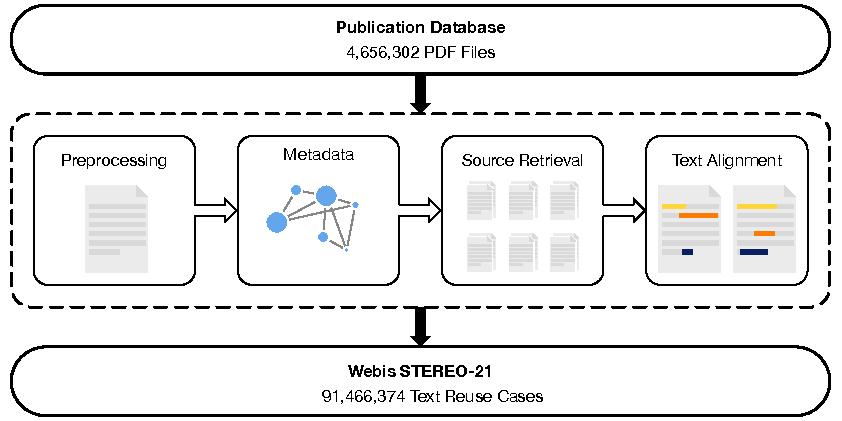
\includegraphics[width=\textwidth]{fig-pipeline}
\caption{Schematic overview of the text reuse detection pipeline. Each document is pre-processed and supplied with metadata. Source retrieval identifies document pairs with local similarities, and alignment is applied to identify reuse cases between those.}
\label{fig:pipeline}
\end{figure}

\begin{figure}[ht]
\centering
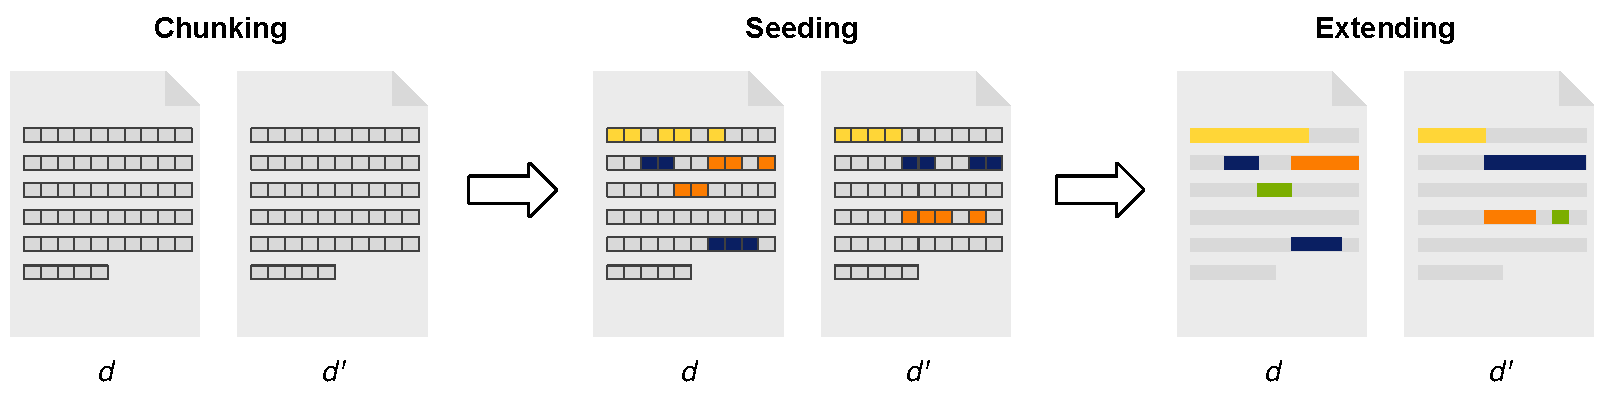
\includegraphics[width=\textwidth]{fig-alignment}
\caption{Schematic overview of the text alignment process. Each document is divided into chunks, matching chunks are identified between documents, and matches are extended to whole reuse cases.}
\label{fig:alignment}
\end{figure}

\begin{table}[ht]
\centering
\small

\caption{Data record overview for case data. \textit{Key} denotes the top-level JSON key by which fields are identified, \textit{Description} provides an explanation of the contained data, and \textit{Type} denotes the data type; ``optional'' indicates fields that can be empty. The text fields are included only in the full version of the corpus.}
\label{tab:data-record-cases}

\begin{tabularx}{\textwidth}{@{}cclXl@{}}
\toprule
& & \textbf{\textsf{Key}} & \textbf{\textsf{Description}} & \textbf{\textsf{Type}} \\

\midrule
& & \texttt{id} & Unique identifier for this case, in UUID format. & String \\

\midrule
\parbox[t]{0.7em}{\multirow{8}{*}{$\left.\rotatebox[origin=c]{90}{\hbox to 24ex{\textit{\textsf{\small\hfill Publication A\hfill}}}}\right\{$}}
%& \parbox[t]{0.7em}{\multirow{3}{*}{\rotatebox[origin=c]{90}{\textit{\textsf{\small Text}}}}}
%& \texttt{text\_a} & Matched text in publication A.& String (full only)\\
%& & \texttt{before\_a} & Text context before the matched text, 100 characters long.& String (full only)\\
%& & \texttt{after\_a} & Text context after the matched text, 100 characters long.& String (full only)\\

%\cmidrule(l){2-5}
& \parbox[t]{0.7em}{\multirow{3}{*}{\rotatebox[origin=c]{90}{\textit{\textsf{\small Locator}}}}}
& \texttt{begin\_a} & Start location of matched text, measured as character offset.& Integer\\
& & \texttt{end\_a} & End location of matched text, measured as character offset.& Integer\\
& & \texttt{doc\_length\_a} & Total length of publication A in characters. & Integer\\

\cmidrule(l){2-5}
& \parbox[t]{0.7em}{\multirow{5}{*}{\rotatebox[origin=c]{90}{\textit{\textsf{\small Context}}}}}
& \texttt{doi\_a} & DOI identifier for publication A.& String\\
& & \texttt{year\_a} & Publication year for publication A.& Integer (optional)\\
& & \texttt{field\_a} & Field(s) of study for publication A.& String Array (optional)\\
& & \texttt{area\_a} & Scientific area(s) for publication A. & String Array (optional)\\
& & \texttt{discipline\_a} & Scientific discipline(s) for publication A.& String Array (optional)\\[1.0ex]

\midrule
\parbox[t]{0.7em}{\multirow{8}{*}{$\left.\rotatebox[origin=c]{90}{\hbox to 24ex{\textit{\textsf{\small\hfill Publication B\hfill}}}}\right\{$}}
%& \parbox[t]{0.7em}{\multirow{3}{*}{\rotatebox[origin=c]{90}{\textit{\textsf{\small Text}}}}}
%& \texttt{text\_b} & Matched text in publication B.& String (full only)\\
%& & \texttt{before\_b} & Text context before the matched text, 100 characters long.& String (full only)\\
%& & \texttt{after\_b} & Text context after the matched text, 100 characters long.& String (full only)\\

%\cmidrule(l){2-5}
& \parbox[t]{0.7em}{\multirow{3}{*}{\rotatebox[origin=c]{90}{\textit{\textsf{\small Locator}}}}}
& \texttt{begin\_b} & Start location of matched text, measured as character offset.& Integer\\
& & \texttt{end\_b} & End location of matched text, measured as character offset.& Integer\\
& & \texttt{doc\_length\_b} & Total length of publication B in characters. & Integer\\

\cmidrule(l){2-5}
& \parbox[t]{0.7em}{\multirow{5}{*}{\rotatebox[origin=c]{90}{\textit{\textsf{\small Context}}}}}
& \texttt{doi\_b} & DOI identifier for publication B.& String\\
& & \texttt{year\_b} & Publication year for publication B.& Integer (optional)\\
& & \texttt{field\_b} & Field(s) of study for publication B.& String Array (optional)\\
& & \texttt{area\_b} & Scientific area(s) for publication B. & String Array (optional)\\
& & \texttt{discipline\_b} & Scientific discipline(s) for publication B.& String Array (optional)\\[1.0ex]

\bottomrule
\end{tabularx}

\end{table}

\begin{table}[ht]
\centering
\small

\caption{Data record overview for publication data. \textit{Key} denotes the top-level JSON key fields are identified by, \textit{Description} provides an explanation of the contained data, and \textit{Type} denotes the data type; ``optional'' indicates fields that can be empty.}
\label{tab:data-record-publications}

\begin{tabularx}{\textwidth}{@{}clXl@{}}
\toprule
& \textbf{\textsf{Key}} & \textbf{\textsf{Description}} & \textbf{\textsf{Type}} \\

\midrule
% \parbox[t]{0.7em}{\multirow{2}{*}{\rotatebox[origin=c]{90}{\textit{\textsf{\small Text}}}}}
% & \texttt{text} & Fulltext of the publication, extracted from its original PDF form. Obtained and processed as described in Section \textit{Data Sources and Preprocessing}. & String \\

%\cmidrule(lr){1-4}
\parbox[t]{0.7em}{\multirow{6}{*}{\rotatebox[origin=c]{90}{\textit{\textsf{\small Metadata}}}}}
& \texttt{doi}         & DOI identifier of the publication.             & String\\
& \texttt{doc\_length} & Total length of the publication in characters. & Integer\\
& \texttt{year}        & Publication year of the publication.           & String Array (optional)\\
& \texttt{field}       & Field of study of the publication.             & String Array (optional)\\
& \texttt{area}        & Scientific area of the publication.            & String Array (optional)\\
& \texttt{discipline}  & Scientific discipline of the publication.      & String Array (optional)\\

\bottomrule
\end{tabularx}

\end{table}

%\begin{table}[th]

\caption{Top-10 detection approaches by teams participating at the PAN Shared Tasks, taken from Potthast et al. (2013)\cite{potthast:2013} and Potthast et al. (2014)\cite{potthast:2014}. Plagdet score, Precision, and Recall by obfuscation strategy and on the complete corpus. Best performing approach per team is listed. Sorted descending by Plagdet score on entire corpus.}
\label{tab:pan13}

\begin{tabularx}{.3\textwidth}{@{}l*{9}{X}}
\toprule
{\bfseries Team}            &  \multicolumn{3}{@{}c@{}}{\bfseries Unobfuscated} & \multicolumn{3}{@{}c@{}}{\bfseries Obfuscated} & \multicolumn{3}{@{}c@{}}{\bfseries Entire Corpus} \\
                            \cmidrule(l@{\tabcolsep}r@{\tabcolsep}){2-4} \cmidrule(l@{\tabcolsep}r@{\tabcolsep}){5-7} \cmidrule(l@{\tabcolsep}r@{\tabcolsep}){8-10} 
                            & {\footnotesize Prec.} & {\footnotesize Rec.} & {\footnotesize Plag.}  & {\footnotesize Prec.} & {\footnotesize Rec.} & {\footnotesize Plag.} & {\footnotesize Prec.} & {\footnotesize Rec.} & {\footnotesize Plag. $\downarrow$} \\

\midrule
Sanchez-Perez (2014)        &         0.83 &   0.98 &    0.90 &       0.93 &   0.76 &    0.80 &      0.88 &   0.88 &    0.88 \\
Oberreuter (2014)           &         0.85 &   1.00 &    0.92 &       0.91 &   0.69 &    0.75 &      0.89 &   0.86 &    0.87 \\
Palkovskii (2014)           &         0.96 &   0.96 &    0.96 &       0.91 &   0.66 &    0.72 &      0.92 &   0.83 &    0.87 \\
Glinos (2014)               &         0.96 &   0.96 &    0.96 &       0.97 &   0.67 &    0.77 &      0.96 &   0.79 &    0.86 \\
Shrestha (2014)             &         0.82 &   0.97 &    0.89 &       0.90 &   0.65 &    0.68 &      0.86 &   0.84 &    0.84 \\
Kong (2012)                 &         0.81 &   0.95 &    0.87 &       0.90 &   0.68 &    0.74 &      0.85 &   0.82 &    0.84 \\
Torrejon (2014)             &         0.90 &   0.97 &    0.93 &       0.92 &   0.58 &    0.68 &      0.90 &   0.77 &    0.83 \\
%Oberreuter (2012)           &         0.89 &   1.00 &    0.94 &       0.91 &   0.54 &    0.62 &      0.89 &   0.77 &    0.83 \\
Gross (2014)                &         0.92 &   0.91 &    0.90 &       0.95 &   0.61 &    0.69 &      0.93 &   0.77 &    0.83 \\
%Torrejon (2013)             &         0.90 &   0.95 &    0.93 &       0.91 &   0.57 &    0.67 &      0.89 &   0.76 &    0.82 \\
%Kong (2014)                 &         0.79 &   0.90 &    0.84 &       0.89 &   0.68 &    0.73 &      0.84 &   0.81 &    0.82 \\
%Kong (2013)                 &         0.76 &   0.91 &    0.83 &       0.89 &   0.68 &    0.73 &      0.83 &   0.81 &    0.82 \\
%Palkovskii (2012)           &         0.79 &   0.99 &    0.88 &       0.87 &   0.58 &    0.65 &      0.82 &   0.76 &    0.79 \\
%Torrejon (2012)             &         0.81 &   0.96 &    0.88 &       0.85 &   0.57 &    0.66 &      0.83 &   0.75 &    0.79 \\
Suchomel (2013)             &         0.69 &   1.00 &    0.82 &       0.75 &   0.65 &    0.70 &      0.73 &   0.77 &    0.74 \\
%Suchomel (2012)             &         0.82 &   1.00 &    0.90 &       0.87 &   0.47 &    0.61 &      0.84 &   0.65 &    0.73 \\
Saremi (2013)               &         0.83 &   0.95 &    0.85 &       0.91 &   0.57 &    0.53 &      0.87 &   0.77 &    0.70 \\
%Shrestha (2013)             &         0.81 &   1.00 &    0.89 &       0.91 &   0.54 &    0.52 &      0.87 &   0.74 &    0.70 \\
Abnar (2014)                &         0.75 &   0.99 &    0.85 &       0.84 &   0.36 &    0.46 &      0.77 &   0.61 &    0.67 \\
Alvi (2014)                 &         0.92 &   0.99 &    0.93 &       0.93 &   0.30 &    0.41 &      0.93 &   0.55 &    0.66 \\
Kueppers (2012)             &         0.83 &   0.84 &    0.82 &       0.89 &   0.31 &    0.43 &      0.87 &   0.51 &    0.63 \\
%Palkovskii (2013)           &         0.80 &   0.85 &    0.82 &       0.84 &   0.33 &    0.43 &      0.82 &   0.54 &    0.62 \\
Nourian (2013)              &         0.93 &   0.88 &    0.90 &       0.97 &   0.21 &    0.31 &      0.95 &   0.43 &    0.58 \\
\textit{Ours}               &         0.90 &   0.89 &    0.88 &       0.92 &   0.13 &    0.22 &      0.93 &   0.46 &    0.51 \\
Sanchez-Vega (2012)         &         0.40 &   0.74 &    0.52 &       0.45 &   0.42 &    0.41 &      0.40 &   0.56 &    0.46 \\
PAN Baseline (2014)         &         0.89 &   1.00 &    0.93 &       0.96 &   0.05 &    0.07 &      0.93 &   0.34 &    0.42 \\
Gillam (2012)               &         0.88 &   0.87 &    0.88 &       0.97 &   0.01 &    0.03 &      0.89 &   0.27 &    0.41 \\
%Gillam (2013)               &         0.88 &   0.84 &    0.86 &       0.97 &   0.01 &    0.02 &      0.88 &   0.26 &    0.40 \\
%Gillam (2014)               &         0.88 &   0.53 &    0.66 &       0.48 &   0.01 &    0.03 &      0.89 &   0.17 &    0.28 \\
Jayapal (2013)              &         0.92 &   0.86 &    0.39 &       0.85 &   0.16 &    0.15 &      0.88 &   0.38 &    0.27 \\
%Jayapal (2012)              &         0.99 &   0.52 &    0.35 &       0.91 &   0.09 &    0.10 &      0.95 &   0.22 &    0.20 \\

\bottomrule
\end{tabularx}


\end{table}

%\begin{table}[th]

\scriptsize
\setlength{\tabcolsep}{4pt}% Org. 6pt

\caption{Competing detection approaches by teams participating at the PAN Shared Tasks, taken from Potthast et al. (2013)\cite{potthast:2013} and Potthast et al. (2014)\cite{potthast:2014}. Plagdet score, Precision, and Recall by obfuscation strategy and on the complete corpus. Sorted descending by Plagdet score.}
\label{tab:pan13}

\begin{tabularx}{.31\textwidth}{@{}l*{3}{X}}
\multicolumn{4}{c}{\bfseries Unobfuscated} \\
\toprule
Team                & Prec.     & Rec.   & Plag.   \\
\midrule
Glinos (2014)       &         0.96 &   0.96 &    0.96 \\
Palkovskii (2014)   &         0.96 &   0.96 &    0.96 \\
Oberreuter (2012)   &         0.89 &   1.00 &    0.94 \\
PAN Baseline (2014) &         0.89 &   1.00 &    0.93 \\
Torrejon (2014)     &         0.90 &   0.97 &    0.93 \\
Alvi (2014)         &         0.92 &   0.99 &    0.93 \\
Torrejon (2013)     &         0.90 &   0.95 &    0.93 \\
Oberreuter (2014)   &         0.85 &   1.00 &    0.92 \\
Nourian (2013)      &         0.93 &   0.88 &    0.90 \\
Sanchez-Perez (2014)&         0.83 &   0.98 &    0.90 \\
Gross (2014)        &         0.92 &   0.91 &    0.90 \\
Suchomel (2012)     &         0.82 &   1.00 &    0.90 \\
\textbf{Ours}       &         \textbf{0.90} &  \textbf{0.88} &    \textbf{0.89} \\
Shrestha (2013)     &         0.81 &   1.00 &    0.89 \\
Shrestha (2014)     &         0.82 &   0.97 &    0.89 \\
Gillam (2012)       &         0.88 &   0.87 &    0.88 \\
Palkovskii (2012)   &         0.79 &   0.99 &    0.88 \\
Torrejon (2012)     &         0.81 &   0.96 &    0.88 \\
Kong (2012)         &         0.81 &   0.95 &    0.87 \\
Gillam (2013)       &         0.88 &   0.84 &    0.86 \\
Abnar (2014)        &         0.75 &   0.99 &    0.85 \\
Saremi (2013)       &         0.83 &   0.95 &    0.85 \\
Kong (2014)         &         0.79 &   0.90 &    0.84 \\
Kong (2013)         &         0.76 &   0.91 &    0.83 \\
Palkovskii (2013)   &         0.80 &   0.85 &    0.82 \\
Kueppers (2012)     &         0.83 &   0.84 &    0.82 \\
Suchomel (2013)     &         0.69 &   1.00 &    0.82 \\
Gillam (2014)       &         0.88 &   0.53 &    0.66 \\
Sanchez-Vega (2012) &         0.40 &   0.74 &    0.52 \\
Jayapal (2013)      &         0.92 &   0.86 &    0.39 \\
Jayapal (2012)      &         0.99 &   0.52 &    0.35 \\
\bottomrule
\end{tabularx}
 %%%    
\hfill
 %%%
\begin{tabularx}{.31\textwidth}{@{}l*{3}{X}}
\multicolumn{4}{c}{\bfseries Obfuscated} \\
\toprule
Team                & Prec.     & Rec.   & Plag.   \\
\midrule
Sanchez-Perez (2014)&       0.93 &   0.76 &    0.80 \\
Glinos (2014)       &       0.97 &   0.67 &    0.77 \\
Oberreuter (2014)   &       0.91 &   0.69 &    0.75 \\
Kong (2012)         &       0.90 &   0.68 &    0.74 \\
Kong (2013)         &       0.89 &   0.68 &    0.73 \\ %!
Kong (2014)         &       0.89 &   0.68 &    0.73 \\ %!
Palkovskii (2014)   &       0.91 &   0.66 &    0.72 \\
Suchomel (2013)     &       0.75 &   0.65 &    0.70 \\
Gross (2014)        &       0.95 &   0.61 &    0.69 \\
Shrestha (2014)     &       0.90 &   0.65 &    0.68 \\
Torrejon (2014)     &       0.92 &   0.58 &    0.68 \\
Torrejon (2013)     &       0.91 &   0.57 &    0.67 \\ %!
Torrejon (2012)     &       0.85 &   0.57 &    0.66 \\ %!
Palkovskii (2012)   &       0.87 &   0.58 &    0.65 \\ %!
Oberreuter (2012)   &       0.91 &   0.54 &    0.62 \\ %!
Suchomel (2012)     &       0.87 &   0.47 &    0.61 \\ %!
Saremi (2013)       &       0.91 &   0.57 &    0.53 \\
Shrestha (2013)     &       0.91 &   0.54 &    0.52 \\ %!
Abnar (2014)        &       0.84 &   0.36 &    0.46 \\
Kueppers (2012)     &       0.89 &   0.31 &    0.43 \\
Palkovskii (2013)   &       0.84 &   0.33 &    0.43 \\ %!
Sanchez-Vega (2012) &       0.45 &   0.42 &    0.41 \\
Alvi (2014)         &       0.93 &   0.30 &    0.41 \\
Nourian (2013)      &       0.97 &   0.21 &    0.31 \\
\textbf{Ours}       &       \textbf{0.92} &   \textbf{0.13} &    \textbf{0.22} \\
Jayapal (2013)      &       0.85 &   0.16 &    0.15 \\
Jayapal (2012)      &       0.91 &   0.09 &    0.10 \\ %!
PAN Baseline (2014) &       0.96 &   0.05 &    0.07 \\
Gillam (2014)       &       0.48 &   0.01 &    0.03 \\
Gillam (2012)       &       0.97 &   0.01 &    0.03 \\ %!
Gillam (2013)       &       0.97 &   0.01 &    0.02 \\ %!
\bottomrule
\end{tabularx}
 %%%    
\hfill
 %%%    
\begin{tabularx}{.31\textwidth}{@{}l*{3}{X}}
\multicolumn{4}{c}{\bfseries Entire Corpus} \\
\toprule
Team                & Prec.     & Rec.   & Plag.   \\
\midrule
Sanchez-Perez (2014)&      0.88 &   0.88 &    0.88 \\
Oberreuter (2014)   &      0.89 &   0.86 &    0.87 \\
Palkovskii (2014)   &      0.92 &   0.83 &    0.87 \\
Glinos (2014)       &      0.96 &   0.79 &    0.86 \\
Shrestha (2014)     &      0.86 &   0.84 &    0.84 \\
Kong (2012)         &      0.85 &   0.82 &    0.84 \\
Torrejon (2014)     &      0.90 &   0.77 &    0.83 \\
Oberreuter (2012)   &      0.89 &   0.77 &    0.83 \\ %!
Gross (2014)        &      0.93 &   0.77 &    0.83 \\
Torrejon (2013)     &      0.89 &   0.76 &    0.82 \\ %!
Kong (2014)         &      0.84 &   0.81 &    0.82 \\ %!
Kong (2013)         &      0.83 &   0.81 &    0.82 \\ %!
Palkovskii (2012)   &      0.82 &   0.76 &    0.79 \\ %!
Torrejon (2012)     &      0.83 &   0.75 &    0.79 \\ %!
Suchomel (2013)     &      0.73 &   0.77 &    0.74 \\
Suchomel (2012)     &      0.84 &   0.65 &    0.73 \\ %!
Saremi (2013)       &      0.87 &   0.77 &    0.70 \\
Shrestha (2013)     &      0.87 &   0.74 &    0.70 \\ %!
Abnar (2014)        &      0.77 &   0.61 &    0.67 \\
Alvi (2014)         &      0.93 &   0.55 &    0.66 \\
Kueppers (2012)     &      0.87 &   0.51 &    0.63 \\
Palkovskii (2013)   &      0.82 &   0.54 &    0.62 \\ %!
Nourian (2013)      &      0.95 &   0.43 &    0.58 \\
\textbf{Ours}       &      \textbf{0.93} &   \textbf{0.46} &    \textbf{0.51} \\
Sanchez-Vega (2012) &      0.40 &   0.56 &    0.46 \\
PAN Baseline (2014) &      0.93 &   0.34 &    0.42 \\
Gillam  (2012)      &      0.89 &   0.27 &    0.41 \\
Gillam  (2013)      &      0.88 &   0.26 &    0.40 \\ %!
Gillam  (2014)      &      0.89 &   0.17 &    0.28 \\ %!
Jayapal (2013)      &      0.88 &   0.38 &    0.27 \\
Jayapal (2012)      &      0.95 &   0.22 &    0.20 \\ %!
\bottomrule
\end{tabularx}

\end{table}

%\begin{table}[th]

\scriptsize
\setlength{\tabcolsep}{4pt}% Org. 6pt

\caption{Competing detection approaches by teams participating at the PAN Shared Tasks, taken from Potthast et al. (2013)\cite{potthast:2013} and Potthast et al. (2014)\cite{potthast:2014}. Plagdet score, Precision, and Recall by obfuscation strategy and on the complete corpus. Sorted descending by Plagdet score.}
\label{tab:pan13}
    
\begin{tabularx}{.31\textwidth}{@{}l*{3}{X}}
\multicolumn{4}{c}{\bfseries Unobfuscated} \\
\toprule
Team                & Prec.     & Rec.   & $F_1$   \\
\midrule
Glinos (2014)        &         0.96 &   0.96 &  0.96 \\
Palkovskii (2014)    &         0.96 &   0.96 &  0.96 \\
Alvi (2014)          &         0.92 &   0.99 &  0.95 \\
Oberreuter (2012)    &         0.89 &   1.00 &  0.94 \\
Baseline (2014)      &         0.89 &   1.00 &  0.94 \\
Torrejon (2014)      &         0.90 &   0.97 &  0.93 \\
Torrejon (2013)      &         0.90 &   0.95 &  0.93 \\
Oberreuter (2014)    &         0.85 &   1.00 &  0.92 \\
Gross (2014)         &         0.92 &   0.91 &  0.91 \\
Nourian (2013)       &         0.93 &   0.88 &  0.90 \\
Sanchez-Perez (2014) &         0.83 &   0.98 &  0.90 \\
Suchomel (2012)      &         0.82 &   1.00 &  0.90 \\
Shrestha (2013)      &         0.81 &   1.00 &  0.89 \\
Shrestha (2014)      &         0.82 &   0.97 &  0.89 \\
Jayapal (2013)       &         0.92 &   0.86 &  0.89 \\
\textbf{Ours}          &         \textbf{0.88} &   \textbf{0.90} &  \textbf{0.89} \\
Saremi (2013)        &         0.83 &   0.95 &  0.89 \\
Torrejon (2012)      &         0.81 &   0.96 &  0.88 \\
Palkovskii (2012)    &         0.79 &   0.99 &  0.88 \\
Gillam (2012)        &         0.88 &   0.87 &  0.88 \\
Kong (2012)          &         0.81 &   0.95 &  0.87 \\
Gillam (2013)        &         0.88 &   0.84 &  0.86 \\
Abnar (2014)         &         0.75 &   0.99 &  0.85 \\
Kong (2014)          &         0.79 &   0.90 &  0.84 \\
Kueppers (2012)      &         0.83 &   0.84 &  0.84 \\
Kong (2013)          &         0.76 &   0.91 &  0.83 \\
Palkovskii (2013)    &         0.80 &   0.85 &  0.82 \\
Suchomel (2013)      &         0.69 &   1.00 &  0.82 \\
Jayapal (2012)       &         0.99 &   0.52 &  0.68 \\
Gillam (2014)        &         0.88 &   0.53 &  0.66 \\
Sanchez-Vega (2012)  &         0.40 &   0.74 &  0.52 \\
\bottomrule
\end{tabularx}
 %%%
\hfill
 %%%
\begin{tabularx}{.31\textwidth}{@{}l*{3}{X}}
\multicolumn{4}{c}{\bfseries Obfuscated} \\
\toprule
Team                 & Prec.      & Rec.   & $F_1$   \\
\midrule
Sanchez-Perez (2014) &       0.93 &   0.76 &  0.83 \\
Glinos (2014)        &       0.97 &   0.67 &  0.79 \\
Oberreuter (2014)    &       0.91 &   0.69 &  0.79 \\
Kong (2012)          &       0.90 &   0.68 &  0.77 \\
Kong (2013)          &       0.89 &   0.68 &  0.77 \\
Kong (2014)          &       0.89 &   0.68 &  0.77 \\
Palkovskii (2014)    &       0.91 &   0.66 &  0.77 \\
Shrestha (2014)      &       0.90 &   0.65 &  0.76 \\
Gross (2014)         &       0.95 &   0.61 &  0.74 \\
Torrejon (2014)      &       0.92 &   0.58 &  0.71 \\
Torrejon (2013)      &       0.91 &   0.57 &  0.70 \\
Saremi (2013)        &       0.91 &   0.57 &  0.70 \\
Suchomel (2013)      &       0.75 &   0.65 &  0.70 \\
Palkovskii (2012)    &       0.87 &   0.58 &  0.70 \\
Torrejon (2012)      &       0.85 &   0.57 &  0.68 \\
Oberreuter (2012)    &       0.91 &   0.54 &  0.68 \\
Shrestha (2013)      &       0.91 &   0.54 &  0.68 \\
Suchomel (2012)      &       0.87 &   0.47 &  0.61 \\
Abnar (2014)         &       0.84 &   0.36 &  0.50 \\
Palkovskii (2013)    &       0.84 &   0.33 &  0.47 \\
Kueppers (2012)      &       0.89 &   0.31 &  0.46 \\
Alvi (2014)          &       0.93 &   0.30 &  0.46 \\
Sanchez-Vega (2012)  &       0.45 &   0.42 &  0.44 \\
Nourian (2013)       &       0.97 &   0.21 &  0.34 \\
Jayapal (2013)       &       0.85 &   0.16 &  0.27 \\
\textbf{Ours}          &       \textbf{0.92} &   \textbf{0.12} &  \textbf{0.22} \\
Jayapal (2012)       &       0.91 &   0.09 &  0.16 \\
Baseline (2014)      &       0.96 &   0.05 &  0.10 \\
Gillam (2014)        &       0.48 &   0.01 &  0.03 \\
Gillam (2012)        &       0.97 &   0.01 &  0.03 \\
Gillam (2013)        &       0.97 &   0.01 &  0.02 \\
\bottomrule
\end{tabularx}
 %%%
\hfill
 %%%
\begin{tabularx}{.31\textwidth}{@{}l*{3}{X}}
\multicolumn{4}{c}{\bfseries Entire Corpus} \\
\toprule
Team                & Prec.     & Rec.   & $F_1$   \\
\midrule
Sanchez-Perez (2014) &      0.88 &   0.88 &  0.88 \\
Palkovskii (2014)    &      0.92 &   0.83 &  0.87 \\
Oberreuter (2014)    &      0.89 &   0.86 &  0.87 \\
Glinos (2014)        &      0.96 &   0.79 &  0.87 \\
Shrestha (2014)      &      0.86 &   0.84 &  0.85 \\
Gross (2014)         &      0.93 &   0.77 &  0.84 \\
Kong (2012)          &      0.85 &   0.82 &  0.84 \\
Torrejon (2014)      &      0.90 &   0.77 &  0.83 \\
Oberreuter (2012)    &      0.89 &   0.77 &  0.83 \\
Kong (2014)          &      0.84 &   0.81 &  0.82 \\
Torrejon (2013)      &      0.89 &   0.76 &  0.82 \\
Kong (2013)          &      0.83 &   0.81 &  0.82 \\
Saremi (2013)        &      0.87 &   0.77 &  0.82 \\
Shrestha (2013)      &      0.87 &   0.74 &  0.80 \\
Palkovskii (2012)    &      0.82 &   0.76 &  0.79 \\
Torrejon (2012)      &      0.83 &   0.75 &  0.79 \\
Suchomel (2013)      &      0.73 &   0.77 &  0.74 \\
Suchomel (2012)      &      0.84 &   0.65 &  0.73 \\
Alvi (2014)          &      0.93 &   0.55 &  0.69 \\
Abnar (2014)         &      0.77 &   0.61 &  0.68 \\
Palkovskii (2013)    &      0.82 &   0.54 &  0.65 \\
Kueppers (2012)      &      0.87 &   0.51 &  0.64 \\
\textbf{Ours}        & \textbf{0.93} &   \textbf{0.46} &  \textbf{0.61} \\
Nourian (2013)       &      0.95 &   0.43 &  0.60 \\
Jayapal (2013)       &      0.88 &   0.38 &  0.53 \\
Baseline (2014)      &      0.93 &   0.34 &  0.50 \\
Sanchez-Vega (2012)  &      0.40 &   0.56 &  0.47 \\
Gillam (2012)        &      0.89 &   0.27 &  0.41 \\
Gillam (2013)        &      0.88 &   0.26 &  0.40 \\
Jayapal (2012)       &      0.95 &   0.22 &  0.36 \\
Gillam (2014)        &      0.89 &   0.17 &  0.28 \\
\bottomrule
\end{tabularx}

\end{table}

%\begin{table}[th]

%\scriptsize
\setlength{\tabcolsep}{4pt}% Org. 6pt
\caption{Precision, Recall, and \bscom[Oder noch konservativer 0.25?]{$F_1$}{$F_{0.5}$} score of competing alignment approaches by teams participating at the PAN Shared Tasks, taken from Potthast et al. (2013)\cite{potthast:2013} and Potthast et al. (2014)\cite{potthast:2014}. Sorted descending by \bscom{$F_1$ score}{precision}. \bscom{}{The} Listed approaches are described in detail in the PAN Workshop proceedings \cite{pan:2012,pan:2013,pan:2014}.}
\label{tab:pan13}
\centering
\begin{tabular}{@{}l*{3}{c}}
\multicolumn{4}{c}{\bfseries PAN13 Evaluation Corpus} \\
\toprule
Team                & Precision     & Recall   & $F_1$   \\
\midrule
Sanchez-Perez (2014) &      0.88 &   0.88 &  0.88 \\
Palkovskii (2014)    &      0.92 &   0.83 &  0.87 \\
Oberreuter (2014)    &      0.89 &   0.86 &  0.87 \\
Glinos (2014)        &      0.96 &   0.79 &  0.87 \\
Shrestha (2014)      &      0.86 &   0.84 &  0.85 \\
Gross (2014)         &      0.93 &   0.77 &  0.84 \\
Kong (2012)          &      0.85 &   0.82 &  0.84 \\
Torrejon (2014)      &      0.90 &   0.77 &  0.83 \\
%Oberreuter (2012)    &      0.89 &   0.77 &  0.83 \\
%Kong (2014)          &      0.84 &   0.81 &  0.82 \\
%Torrejon (2013)      &      0.89 &   0.76 &  0.82 \\
%Kong (2013)          &      0.83 &   0.81 &  0.82 \\
Saremi (2013)        &      0.87 &   0.77 &  0.82 \\
%Shrestha (2013)      &      0.87 &   0.74 &  0.80 \\
%Palkovskii (2012)    &      0.82 &   0.76 &  0.79 \\
%Torrejon (2012)      &      0.83 &   0.75 &  0.79 \\
Suchomel (2013)      &      0.73 &   0.77 &  0.74 \\
%Suchomel (2012)      &      0.84 &   0.65 &  0.73 \\
Alvi (2014)          &      0.93 &   0.55 &  0.69 \\
Abnar (2014)         &      0.77 &   0.61 &  0.68 \\
%Palkovskii (2013)    &      0.82 &   0.54 &  0.65 \\
Kueppers (2012)      &      0.87 &   0.51 &  0.64 \\
\textbf{Ours}        &\textbf{0.93} &   \textbf{0.46} &  \textbf{0.61} \\
Nourian (2013)       &      0.95 &   0.43 &  0.60 \\
Jayapal (2013)       &      0.88 &   0.38 &  0.53 \\
Baseline (2014)      &      0.93 &   0.34 &  0.50 \\
Sanchez-Vega (2012)  &      0.40 &   0.56 &  0.47 \\
Gillam (2012)        &      0.89 &   0.27 &  0.41 \\
%Gillam (2013)        &      0.88 &   0.26 &  0.40 \\
%Jayapal (2012)       &      0.95 &   0.22 &  0.36 \\
%Gillam (2014)        &      0.89 &   0.17 &  0.28 \\
\bottomrule
\end{tabular}

\end{table}


\begin{table}[th]

%\scriptsize
\setlength{\tabcolsep}{4pt}% Org. 6pt
\caption{Precision, Recall, and $F_{0.5}$ score of competing alignment approaches by teams participating at the PAN Shared Tasks, taken from Potthast et al. (2013)\cite{potthast:2013} and Potthast et al. (2014)\cite{potthast:2014} and sorted descending by precision. The listed approaches are described in detail in the PAN Workshop proceedings \cite{pan:2012,pan:2013,pan:2014}. Complexity denotes the runtime complexity of the approach; Data Specificity denotes the degree of PAN-specific optimizations reducing transferability to other data domains, i.e. ensemble methods, trained approaches, feature extraction, or special handling of corpus characteristics.}
\label{tab:pan13}

\centering
\begin{tabular}{@{}l*{3}{c}cc@{}}
\multicolumn{6}{c}{\bfseries PAN13 Evaluation Corpus} \\
\toprule
Team                    & Precision$\downarrow$ & Recall        & $F_{0.5}$         & Complexity    & Data Specificity  \\
\midrule
        Glinos (2014)   &       0.96            &    0.79       &  0.92             & $O(nm)$       & Medium            \\
       Jayapal (2012)   &       0.95            &    0.22       &  0.57             & $O(n+m)$      & Low               \\
       Nourian (2013)   &       0.95            &    0.43       &  0.76             & ---           & ---               \\
         Gross (2014)   &       0.93            &    0.77       &  0.89             & $O(nm)$       & Low               \\
         Alvi (2014)    &       0.93            &    0.55       &  0.82             & $O(n+m)$      & Medium            \\
        \textbf{Ours}   &\textbf{0.93}          &\textbf{0.46}  &  \textbf{0.77}    & $O(n+m)$      & Low               \\
      Baseline (2014)   &       0.93            &    0.34       &  0.69             & $O(n+m)$      & Low               \\
    Palkovskii (2014)   &       0.92            &    0.83       &  0.90             & $O(nm)$       & High              \\
      Torrejon (2014)   &       0.90            &    0.77       &  0.87             & $O(nm)$       & High              \\
        Gillam (2014)   &       0.89            &    0.17       &  0.48             & $O(nm)$       & High              \\ %
    Oberreuter (2014)   &       0.89            &    0.86       &  0.88             & ---           & ---               \\
    Oberreuter (2012)   &       0.89            &    0.77       &  0.86             & ---           & ---               \\ %
        Gillam (2012)   &       0.89            &    0.27       &  0.61             & $O(nm)$       & High              \\ %
      Torrejon (2013)   &       0.89            &    0.76       &  0.86             & $O(nm)$       & High              \\ %
        Gillam (2013)   &       0.88            &    0.26       &  0.60             & $O(nm)$       & High              \\ %
       Jayapal (2013)   &       0.88            &    0.38       &  0.70             & $O(n+m)$      & Low               \\
 Sanchez-Perez (2014)   &       0.88            &    0.88       &  0.88             & $O(nm)$       & High              \\
      Kueppers (2012)   &       0.87            &    0.51       &  0.76             & $O(nm)$       & Low               \\
      Shrestha (2013)   &       0.87            &    0.74       &  0.84             & $O(nm)$       & Medium            \\
        Saremi (2013)   &       0.87            &    0.77       &  0.85             & ---           & ---               \\
      Shrestha (2014)   &       0.86            &    0.84       &  0.86             & $O(nm)$       & Medium            \\
          Kong (2012)   &       0.85            &    0.82       &  0.84             & $O(nm)$       & Low               \\
      Suchomel (2012)   &       0.84            &    0.65       &  0.79             & $O(n+m)$      & Medium            \\
          Kong (2014)   &       0.84            &    0.81       &  0.83             & $O(nm)$       & Low               \\
          Kong (2013)   &       0.83            &    0.81       &  0.83             & $O(nm)$       & Low               \\
      Torrejon (2012)   &       0.83            &    0.75       &  0.81             & $O(nm)$       & High              \\ %
    Palkovskii (2013)   &       0.82            &    0.54       &  0.74             & $O(nm)$       & High              \\
    Palkovskii (2012)   &       0.82            &    0.76       &  0.81             & $O(nm)$       & High              \\
         Abnar (2014)   &       0.77            &    0.61       &  0.73             & $O(nm)$       & Medium            \\
      Suchomel (2013)   &       0.73            &    0.77       &  0.74             & $O(n+m)$      & Medium            \\
  Sanchez-Vega (2012)   &       0.40            &    0.56       &  0.42             & $O(nm)$       & Medium            \\
\bottomrule
\end{tabular}

\end{table}


%\begin{table}[th]

\caption{Top-10 detection approaches by teams participating at the PAN Shared Tasks, taken from Potthast et al. (2013)\cite{potthast:2013} and Potthast et al. (2014)\cite{potthast:2014}. Plagdet score, Precision, and Recall by obfuscation strategy and on the complete corpus. Best performing approach per team is listed. Sorted descending by Plagdet score on the entire corpus.}
\label{tab:pan13}


\begin{tabularx}{\textwidth}{@{}l*{15}{X}}
\toprule
{\bfseries Team} & \multicolumn{12}{@{}c@{}}{\bfseries Performance by Obfuscation Strategy} & \multicolumn{3}{@{}c@{}}{\bfseries Entire Corpus} \\

\cmidrule(l@{\tabcolsep}r@{\tabcolsep}){2-13}
& \multicolumn{3}{@{}c@{}}{None} & \multicolumn{3}{@{}c@{}}{ Random} & \multicolumn{3}{@{}c@{}}{Translation} & \multicolumn{3}{@{}c@{}}{Summary} \\

\cmidrule(l@{\tabcolsep}r@{\tabcolsep}){2-4} \cmidrule(l@{\tabcolsep}r@{\tabcolsep}){5-7} \cmidrule(l@{\tabcolsep}r@{\tabcolsep}){8-10} \cmidrule(l@{\tabcolsep}r@{\tabcolsep}){11-13} \cmidrule(l@{\tabcolsep}r@{\tabcolsep}){14-16} 
& {\footnotesize Plag.} & {\footnotesize Prec.} & {\footnotesize Rec.}  & {\footnotesize Plag.} & {\footnotesize Prec.} & {\footnotesize Rec.}  & {\footnotesize Plag.} & {\footnotesize Prec.} & {\footnotesize Rec.}  & {\footnotesize Plag.} & {\footnotesize Prec.} & {\footnotesize Rec.} & {\footnotesize Plag.} & {\footnotesize Prec.} & {\footnotesize Rec.} \\
\midrule
%\textsuperscript{\dag}Kong (2012)               & 0.87 & 0.80 & 0.94 & 0.83 & 0.89 & 0.77 & 0.85 & 0.85 & 0.85 & 0.43 & 0.96 & 0.29 & 0.83 & 0.85 & \textbf{0.82} \\
%\textsuperscript{\dag}Oberreuter (2012)         & 0.91 & 0.89 & 0.99 & 0.86 & 0.87 & 0.65 & 0.84 & 0.90 & 0.79 & 0.13 & 0.98 & 0.07 & 0.82 & 0.89 & 0.76 \\
%\textsuperscript{\dag}R.\ Torrej{\'o}n (2013)   & 0.92 & 0.90 & 0.95 & 0.74 & 0.90 & 0.63 & 0.85 & 0.89 & 0.81 & 0.34 & 0.90 & 0.21 & 0.82 & 0.89 & 0.76 \\
%\textsuperscript{\textdagger}Kong (2013)       & 0.82 & 0.76 & 0.90 & 0.82 & 0.89 & 0.78 & 0.85 & 0.85 & 0.84 & 0.43 & 0.96 & 0.30 & 0.81 & 0.82 & 0.81 \\
%\textsuperscript{\dag}Palkovskii (2012)         & 0.88 & 0.79 & 0.99 & 0.79 & 0.84 & 0.75 & 0.74 & 0.83 & 0.66 & 0.27 & 0.94 & 0.16 & 0.79 & 0.82 & 0.76 \\
%\textsuperscript{\textdagger}R.\ Torrej{\'o}n (2012)     & 0.88 & 0.81 & 0.96 & 0.70 & 0.83 & 0.60 & 0.80 & 0.81 & 0.79 & 0.44 & 0.92 & 0.29 & 0.78 & 0.82 & 0.75 \\
%\textsuperscript{\textdagger}Suchomel (2012)   & 0.89 & 0.81 & 0.99 & 0.65 & 0.87 & 0.51 & 0.63 & 0.85 & 0.50 & 0.50 & 0.87 & 0.35 & 0.73 & 0.84 & 0.64 \\
%\textsuperscript{\dag}Shrestha (2013)           & 0.89 & 0.80 & 0.99 & 0.66 & 0.92 & 0.71 & 0.62 & 0.88 & 0.63 & 0.11 & 0.90 & 0.09 & 0.69 & 0.87 & 0.73 \\
%\textsuperscript{\dag}Kueppers (2012)           & 0.81 & 0.83 & 0.83 & 0.51 & 0.89 & 0.36 & 0.56 & 0.89 & 0.36 & 0.13 & 0.86 & 0.42 & 0.62 & 0.86 & 0.51 \\
%\textsuperscript{\textdagger}Palkovskii (2013) & 0.82 & 0.79 & 0.85 & 0.49 & 0.93 & 0.36 & 0.60 & 0.82 & 0.42 & 0.09 & 0.67 & 0.08 & 0.61 & 0.81 & 0.53 \\
%\textsuperscript{\dag}Nourian (2013)            & 0.90 & 0.92 & 0.87 & 0.35 & 0.96 & 0.23 & 0.43 & 0.95 & 0.28 & 0.11 & 0.99 & 0.07 & 0.57 & 0.94 & 0.43 \\
%\textsuperscript{\dag}S{\'a}nchez-Vega (2012)   & 0.52  & 0.40  & 0.74  & 0.45  & 0.49  & 0.43  & 0.44  & 0.37  & 0.58  & 0.28  & 0.45  & 0.22  & 0.45  & 0.39  & 0.56  \\

Sanchez-Perez (2014)\cite{sanchezperez:2014}        & 0.90  & 0.83  & 0.97  & 0.88  & 0.91  & 0.86  & 0.88  & 0.88  & 0.88  & 0.56  & 0.99  & 0.41  & 0.87  & 0.99  & 0.87  \\
Oberreuter (2014)\cite{oberreuter:2014}             & 0.91  & 0.85  & 0.99  & 0.86  & 0.90  & 0.83  & 0.88  & 0.89  & 0.85  & 0.36  & 0.89  & 0.24  & 0.86  & 0.93  & 0.85  \\
Palkovskii (2014)\cite{palkovskii:2014}             & 0.96  & 0.95  & 0.96  & 0.86  & 0.91  & 0.82  & 0.85  & 0.89  & 0.82  & 0.27  & 0.91  & 0.17  & 0.86  & 0.91  & 0.82  \\
Glinos (2014)\cite{glinos:2014}                     & 0.96  & 0.96  & 0.96  & 0.80  & 0.96  & 0.72  & 0.84  & 0.96  & 0.76  & 0.62  & 0.96  & 0.48  & 0.85  & 0.94  & 0.79  \\
Shrestha (2014)\cite{shrestha:2014}                 & 0.89  & 0.80  & 0.97  & 0.86  & 0.91  & 0.83  & 0.84  & 0.84  & 0.85  & 0.15  & 0.93  & 0.08  & 0.84  & 0.85  & 0.83  \\
Kong (2012)\cite{kong:2012}                         & 0.87  & 0.80  & 0.94  & 0.83  & 0.89  & 0.77  & 0.85  & 0.85  & 0.85  & 0.43  & 0.96  & 0.29  & 0.83  & 0.85  & 0.82  \\
R.\ Torrej{\'o}n (2013)\cite{rodrigueztorrejon:2014}& 0.93  & 0.90  & 0.95  & 0.75  & 0.90  & 0.63  & 0.85  & 0.85  & 0.81  & 0.35  & 0.90  & 0.21  & 0.82  & 0.89  & 0.76  \\
Gross (2014)\cite{gross:2014}                       & 0.89  & 0.91  & 0.90  & 0.80  & 0.96  & 0.71  & 0.83  & 0.92  & 0.78  & 0.31  & 0.94  & 0.20  & 0.82  & 0.93  & 0.76  \\
Suchomel (2013)\cite{suchomel:2014}                 & 0.81  & 0.69  & 0.99  & 0.75  & 0.82  & 0.68  & 0.67  & 0.68  & 0.66  & 0.61  & 0.67  & 0.56  & 0.74  & 0.72  & 0.76  \\
Saremi (2013)\cite{saremi:2013}                     & 0.84  & 0.82  & 0.95  & 0.65  & 0.91  & 0.68  & 0.70  & 0.84  & 0.80  & 0.11  & 0.94  & 0.10  & 0.69  & 0.86  & 0.77  \\

\midrule
\textit{Ours}                                       & 0.89  & 0.88  & 0.90  & 0.20  & 0.90  & 0.11  & 0.27  & 0.88  & 0.16  & 0.18  & 0.99  & 0.10  & 0.51  & 0.93  & 0.46  \\
%\textit{Ours} (diff. to best)                   & 0.07  & 0.08  & 0.09  & 0.68  & 0.06  & 0.75  & 0.61  & 0.08  & 0.72  & 0.18  & 0.99  & 0.10  & 0.51  & 0.93  & 0.46  \\
%Baseline                                        & 0.93  & 0.88  & 0.99  & 0.07  & 0.98  & 0.04  & 0.10  & 0.97  & 0.08  & 0.04  & 0.91  & 0.03  & 0.42  & 0.92  & 0.34  \\

\bottomrule
\end{tabularx}


\end{table}

\begin{table}[ht]
    \centering
    \caption{Precision, Recall, and $F_{0.5}$ of the text alignment component per obfuscation strategy and on the complete evaluation corpus.}
    \label{tab:evaluation}
    \begin{tabular}{lccc}
    \multicolumn{4}{c}{\bfseries PAN13 Evaluation Corpus} \\
    \toprule
                            &  Precision &  Recall &$F_{0.5}$ \\
    \midrule
    No Obfuscation          &       0.88 &    0.90 &  0.88 \\
    No Plagiarism           &       1.00 &    1.00 &  1.00 \\
    Random Obfuscation      &       0.90 &    0.11 &  0.37 \\
    Summary Obfuscation     &       0.99 &    0.10 &  0.36 \\
    Translation Obfuscation &       0.88 &    0.16 &  0.46 \\ \midrule
    Entire Corpus           &       0.93 &    0.46 &  0.77 \\
    \bottomrule
    \end{tabular}
\end{table}

\end{document}


%%%%%%%%%%%%%%%%%%%%%%%%%%%%%%%%%%%%%%%%%%%%%%%%%%%%%%%%%%%%%%%%%%%%%%%%
